\documentclass{bmstu}


\usepackage{physics}
\usepackage{pdfpages}
\usepackage{tabularx}
\usepackage{longtable}
\usepackage{xfrac}
\usepackage{amssymb}
\usepackage{dsfont}
\usepackage{upgreek}
\usepackage{color, colortbl}
\usepackage{listings}
\usepackage{ amssymb }
\usepackage{tikz}
\usepackage{mathtools}
\usepackage{amsmath}

\graphicspath{
	{graphics/}
}

\begin{document}
\section*{01/11}
\underline{Конечные элементы более высокого порядка}

\underline{Одномерные квадратичные и кубические функции}
\[
\varphi = \alpha_1 + \alpha_2x, \ \dim L = 1, n = 2 \text{ -- симплекс элементы.}
\]

Комплекс элементы -- количество узлов n > 2.  

\begin{center}
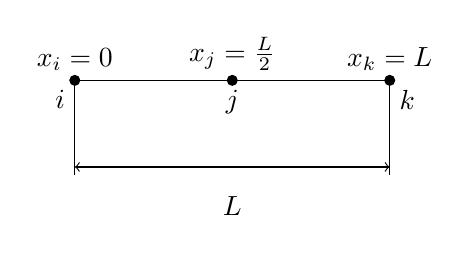
\begin{tikzpicture}[scale=2]
\draw (-1,0) -- (1,0);
\fill (-1,0) circle (1pt) node[below left]{$i$} node[above]{$x_i = 0$};
\fill (0,0) circle (1pt) node[below]{$j$} node[above]{$x_j = \frac{L}{2}$};
\fill (1,0) circle (1pt) node[below right]{$k$} node[above]{$x_k = L$};
\draw (-1,0) -- (-1, -0.6);
\draw (1,0) -- (1, -0.6);
\draw[<->] (-1, -0.55) -- (1, -0.55);
\node at (0, -0.8) {$L$};
\end{tikzpicture}
\end{center}

$\varphi = \alpha_1 + \alpha_2x + \alpha_3x^2 = N \Phi$

В общем виде: $\varphi = \alpha_1 + \alpha_2x + \cdots + \alpha_nx^{n-1}$
\[
\begin{cases}
\Phi_i = \alpha_1 + \alpha_2x_i + \alpha_2x^{2}_i \\
\Phi_j = \alpha_1 + \alpha_2x_j + \alpha_2x^{2}_j \\
\Phi_k = \alpha_1 + \alpha_2x_k + \alpha_2x^{2}_k \\
\end{cases}
\rightarrow \alpha_1, \alpha_2, \alpha_3
\]
\[
\alpha_1 = \Phi_i, \ \alpha_2 = \frac{-3\Phi_i + 4\Phi_j -\Phi_k}{L}, \ \alpha_3 = \frac{2(\Phi_i-2\Phi_j+\Phi_k)}{L^2}
\]
\[
\varphi = \alpha_1 + \alpha_2x + \alpha_3x^2 = 
\]
\[
 = \Phi_i   \underbrace{\left(1 - \frac{3x}{L} + \frac{2x^2}{L^2} \right) }_{N_i}   + \Phi_j \underbrace{\left(\frac{4x}{L} - \frac{4x^2}{L^2} \right)}_{N_j} + \Phi_k \underbrace{\left(-\frac{x}{L} + \frac{2x^2}{L^2} \right)}_{N_k} = 
\]
\[
 = N_i \Phi_i + N_j \Phi_j + N_k \Phi_k = [N]\{\Phi\}
\]
\[
N_i = 1 - \frac{3x}{L} + \frac{2x^2}{L^2}, \ N_j = \frac{4x}{L} - \frac{4x^2}{L^2}, \ N_k = -\frac{x}{L} + \frac{2x^2}{L^2}
\]

Этот же результат можно получить без использования системы уравнений. Зададим в узлах пробные функции $f_{\alpha},\ \alpha \in \{i, j, k\}$, такие, что $f_{\alpha}(x_{\alpha}) = 0$:


Формулы для нахождения функций форм без использования системы уравнений: 
\[
N_i = \frac{f_jf_k}{f_jf_k|_{x = x_i}}, \ N_j = \frac{f_if_k}{f_if_k|_{x = x_j}}, \ N_k = \frac{f_if_j}{f_if_j|_{x = x_k}}
\]































\end{document}